%%%%%%%%%%%%%%%%%%%%%%%%%%%%%%%%%%%%%%%%%
% Beamer Presentation
% LaTeX Template
% Version 1.0 (10/11/12)
%
% This template has been downloaded from:
% http://www.LaTeXTemplates.com
%
% License:
% CC BY-NC-SA 3.0 (http://creativecommons.org/licenses/by-nc-sa/3.0/)
%
%%%%%%%%%%%%%%%%%%%%%%%%%%%%%%%%%%%%%%%%%

%----------------------------------------------------------------------------------------
%	PACKAGES AND THEMES
%----------------------------------------------------------------------------------------

\documentclass{beamer}

\mode<presentation> {

\usetheme{AnnArbor}

%\setbeamertemplate{navigation symbols}{} % To remove the navigation symbols from the bottom of all slides uncomment this line
}

\usepackage{graphicx} % Allows including images
\usepackage{booktabs} % Allows the use of \toprule, \midrule and \bottomrule in tables
\usepackage{amsmath}
\usepackage{amssymb}
\usepackage{subfigure}
\usepackage{color}
\usepackage{dsfont}
\usepackage{subfigure}


%\newtheorem{example}{Example}
%\newtheorem{definition}{Definition}

\def\ang#1{\left\langle#1\right\rangle}
\def\prob{\mathsf{ProbMeas}}
\def\seq{\mathsf{Sequences}}
\def\X{\mathcal{X}}
\def\Y{\mathcal{Y}}
\def\U{\mathcal{U}}
\def\RR{\mathbb{R}}
\def\power{\mathcal{P}}
\def\less#1{\overset{#1}{\rule{0pt}{4pt}\smash{\preccurlyeq}}}
\def\subs{\subseteq}

%----------------------------------------------------------------------------------------
%	TITLE PAGE
%----------------------------------------------------------------------------------------

\title[Minimal Representation]{Designing Agents with\\ Task-Specific Minimal Representation} % The short title appears at the bottom of every slide, the full title is only on the title page

\author{Joshua Hernandez} % Your name
\institute[UCLA] % Your institution as it will appear on the bottom of every slide, may be shorthan\usepackage{dsfont}d to save space
{
University of California, Los Angeles\\ % Your institution for the title page
\medskip
\textit{jheez@ucla.edu} % Your email address
}
\date{\today} % Date, can be changed to a custom date

\begin{document}

\begin{frame}
\titlepage % Print the title page as the first slide
\end{frame}


\iffalse
%------------------------------------------------
\section{Formalization} % Sections can be created in order to organize your presentation into discrete blocks, all sections and subsections are automatically printed in the table of contents as an overview of the talk
%------------------------------------------------

\subsection{Definitions} % A subsection can be created just before a set of slides with a common theme to further break down your presentation into chunks
%------------------------------------------------


\begin{frame}
\frametitle{Tasks}
\begin{definition}[Task]
A \textbf{task} on the \textbf{state-space} $\X$ is a \emph{partial ordering $\less{T}$ on $\prob(\X)$}
\end{definition}

\begin{itemize}
 \item We can restrict this to $\power(\X)$ (possibilistic) or $\X$ (deterministic).
 \item Given a state-value function $E:\X\to\RR$, and a partial ordering 
 $\less{T}_\RR$ on $\prob(\RR)$, we can derive an ordering
 $$\mu_1\,\less{T}\, \mu_2 \iff (\mu_1\circ E)\,\less{T}_\RR\,(\mu_2\circ E) $$
 for $\mu_1, \mu_2\in\prob(\X)$.  
 We would usually expect $\less{T}_\RR$ to respect stochastic dominance, i.e.
 $$\mu_1\leq\mu_2\implies\mu_1\,\less{T}_\RR\,\mu_2$$
\end{itemize}
\end{frame}

\include{slides.pdf}

%------------------------------------------------

\begin{frame}
\frametitle{Sensor}
\begin{definition}[Sensor]
A \textbf{sensor} on $\X$ is a function $S:\seq(\X)\to\prob(\X)$.\\
A sensor is \textbf{memoryless} if it is a function of the last entry of its sequence.
\end{definition}
In the following, we will only consider memoryless sensors, \
although most of the definitions can be extended to general sensors.
\begin{definition}[Sensor Consistency]
A sensor is \textbf{consistent with} the task $\less{T}_\X$ when
$$ S({x_1})\,\less{T}\,S({x_2}) \implies \delta_{x_1}\,\less{T}\,\delta_{x_2}\qquad\text{for all $x_1,x_2\in\X$,}$$
where $\delta_x(A) := \mathds{1}(x\in A)$ for $x\in\X$ and $A\subs\X$.
\end{definition}
\end{frame}

%------------------------------------------------

\begin{frame}
\frametitle{Sensors, continued}
\begin{definition}[Sensor Refinement]
 A sensor $S_1$ \textbf{is refined by} a sensor $S_2$ with respect to $\less{T}$ when
 $$S_1(x_1)\,\less{T}\,S_2(x_2) \implies S_2(x_1)\,\less{T}\,S_2(x_2)\qquad\text{for all $x_1, x_2\in\X$.}$$
 A \textbf{perfect} sensor $S$ with respect to $\less{T}$ is one such that
 $$\delta_{x_1}\,\less{T}\,\delta_{x_2} \implies S(x_1)\,\less{T}\,S(x_2)\qquad\text{for all $x_1, x_2\in\X$,}$$
 i.e. it satisfies the converse of the consistency condition.
\end{definition}
\end{frame}

 %------------------------------------------------

\begin{frame}
\frametitle{POMDP tasks}
$\ang{\X, \U, \Y, \D, \Omega}$
S is a set of states,
A is a set of actions,
O is a set of observations,
T is a set of conditional transition probabilities,
\Omega is a set of conditional observation probabilities,
R: A \times S \to \mathbb{R} is the reward function.
\end{frame}
\fi

\begin{frame}
\frametitle{Bit-at-a-time (Censi)}
Proposed by Andrea Censi, MIT-LIDS: Greedily separate ambiguous contexts along decision tree.
\begin{figure}
\centering
\subfigure[Decision Tree]{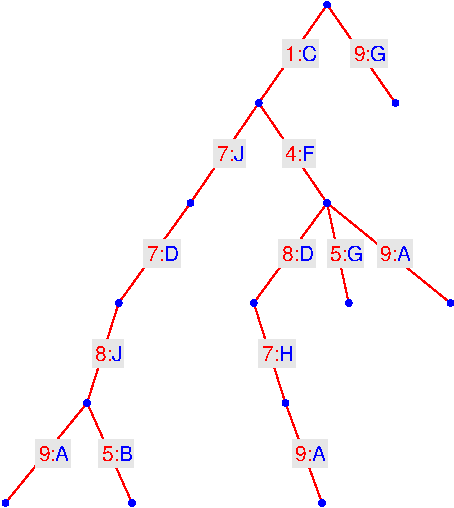
\includegraphics[height=2in]{cdiag1}}$\quad\phantom{\to}\quad$
\phantom{\subfigure[Reduced FSM]{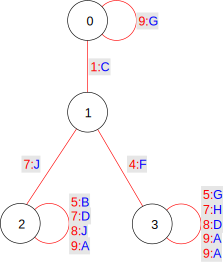
\includegraphics[trim=0in -2in 0in 0in, width=1.5in]{cdiag3}}}
\end{figure}
\end{frame}
 
 \setcounter{subfigure}{0}
 
\begin{frame}
\frametitle{Bit-at-a-time (Censi)}
Proposed by Andrea Censi, MIT-LIDS: Greedily separate ambiguous contexts along decision tree.
\begin{figure}
\centering
\subfigure[Decision Tree]{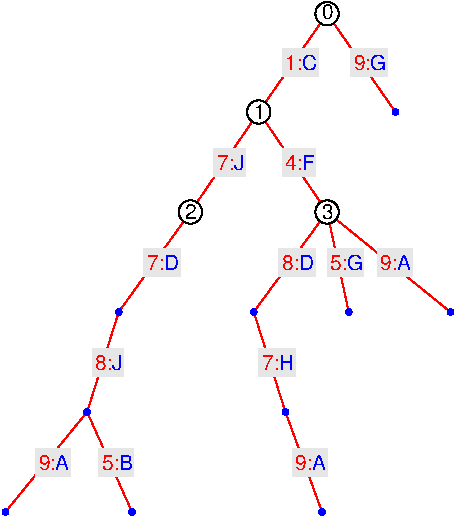
\includegraphics[height=2in]{cdiag2}}$\quad\phantom{\to}\quad$
\phantom{\subfigure[Reduced FSM]{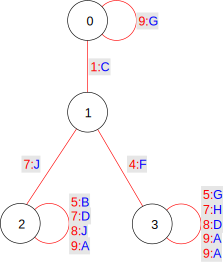
\includegraphics[trim=0in -2in 0in 0in, width=1.5in]{cdiag3}}}
\end{figure}
\end{frame}

\setcounter{subfigure}{0}

\begin{frame}
\frametitle{Bit-at-a-time (Censi)}
Proposed by Andrea Censi, MIT-LIDS: Greedily separate ambiguous contexts along decision tree.
\begin{figure}
\centering
\subfigure[Decision Tree]{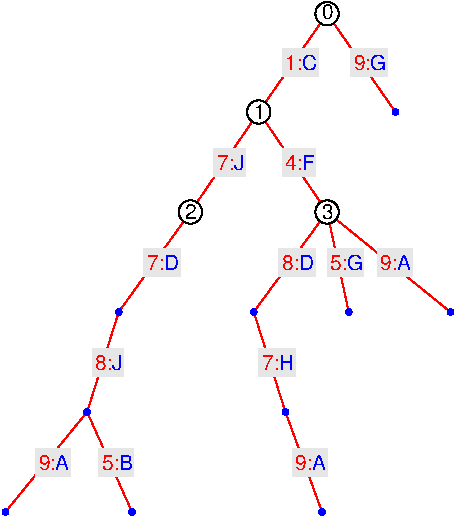
\includegraphics[height=2in]{cdiag2}}$\quad\phantom{\to}\quad$
\subfigure[Reduced FSM]{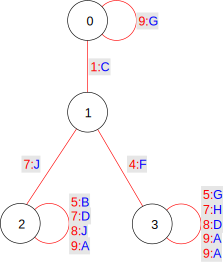
\includegraphics[trim=0in -2in 0in 0in, width=1.5in]{cdiag3}}
\end{figure}
\end{frame}

\begin{frame}
\frametitle{Greedy Clique Covering}
Greedily combine compatible states
\begin{figure}
\centering
\subfigure[Decision Tree]{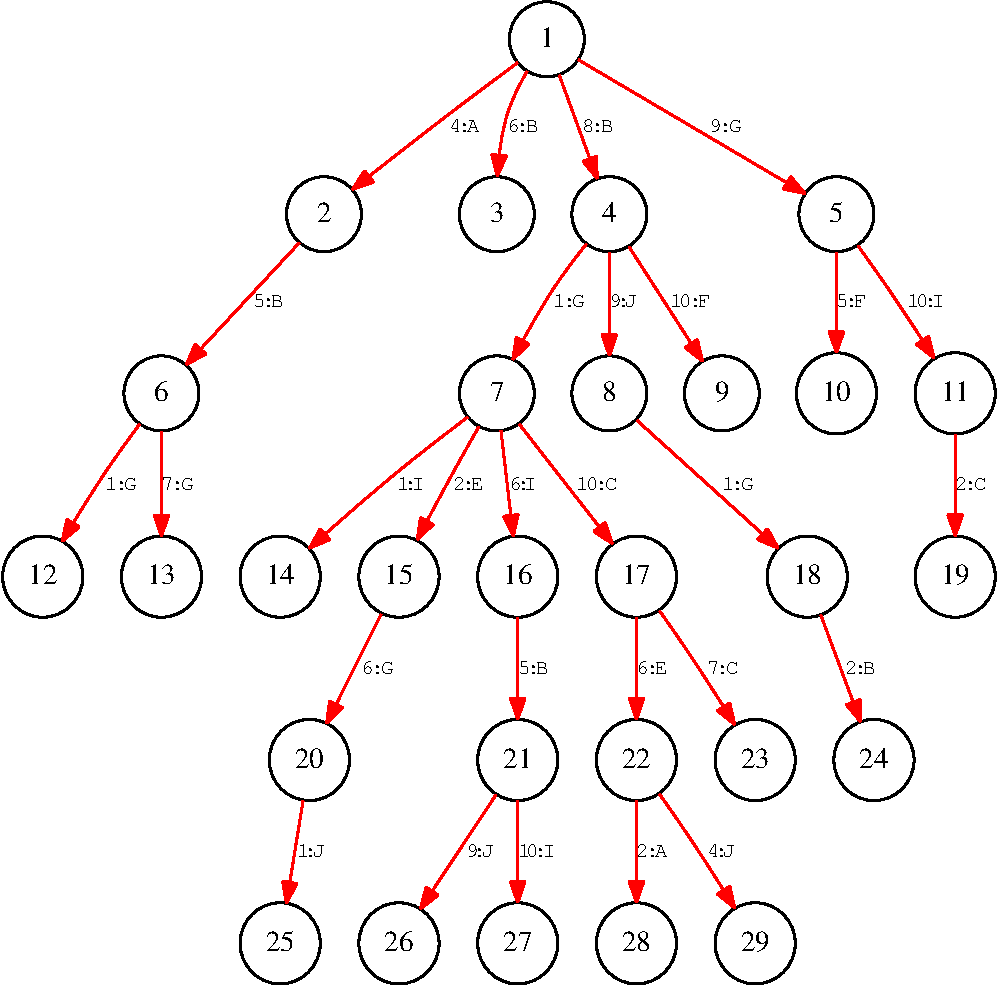
\includegraphics[height=2in]{random_alg-1}}$\quad\phantom{\to}\quad$
\subfigure[Compatibility Matrix]{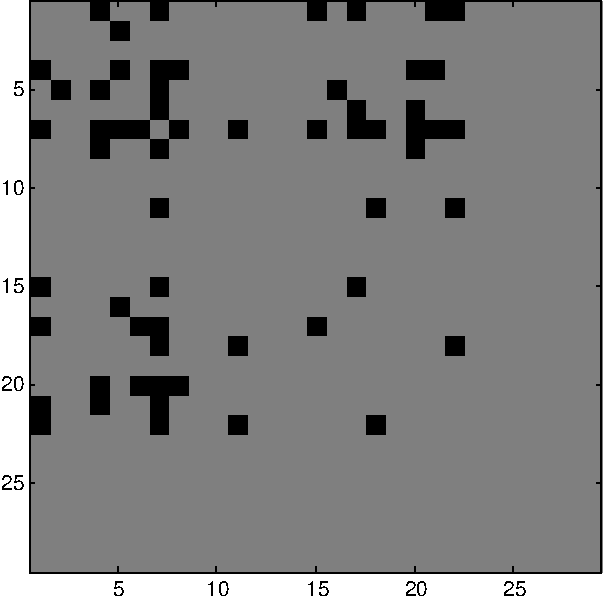
\includegraphics[height=2in]{random_adj}}
\end{figure}
\end{frame}

\begin{frame}
\frametitle{Greedy Clique Covering}
Greedily combine compatible states
\begin{figure}
\centering
\subfigure[Greedy Clique Covering]{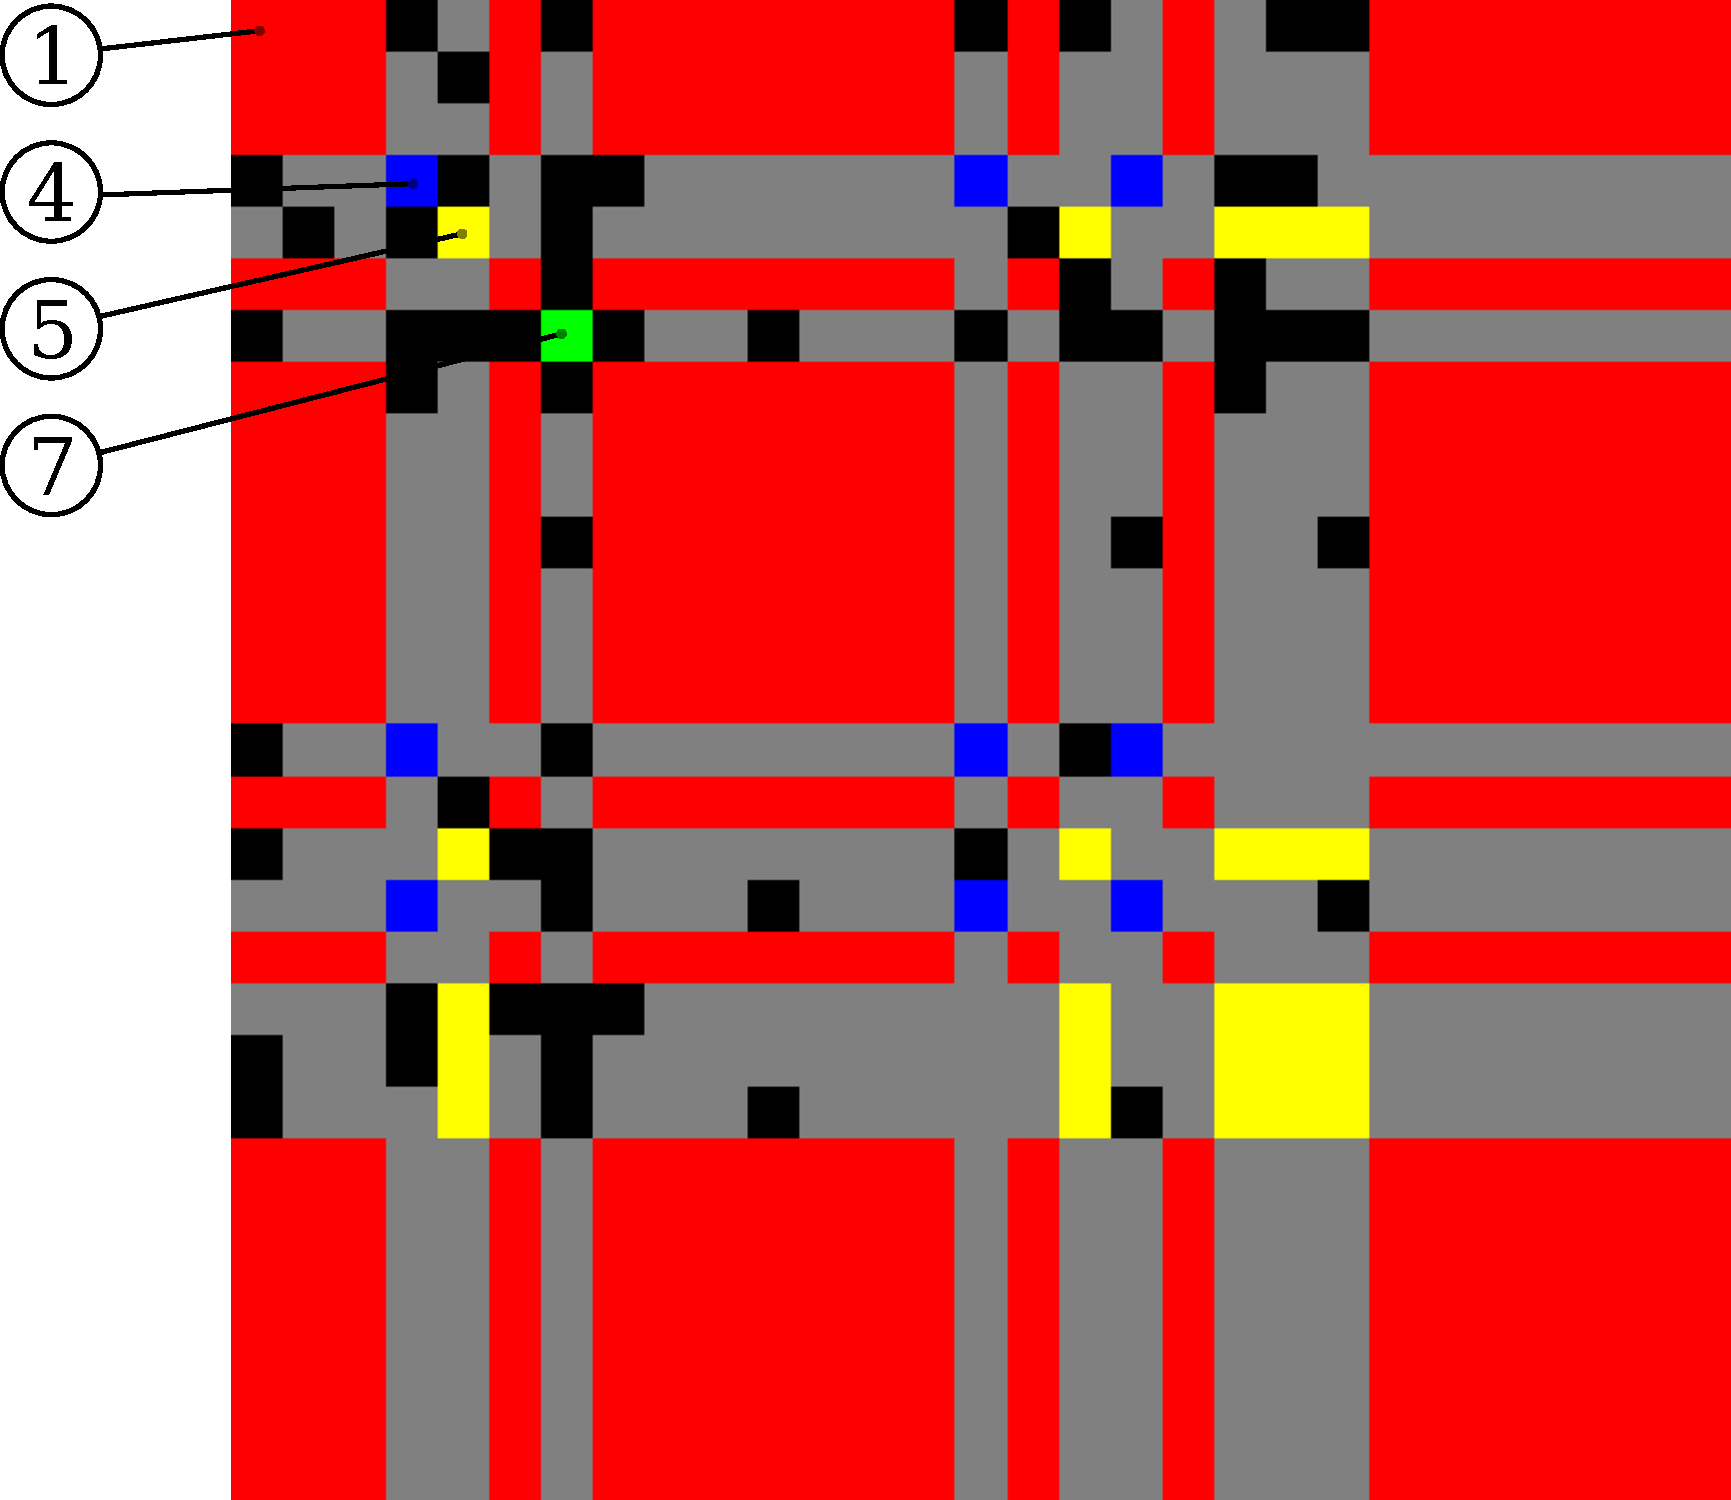
\includegraphics[height=2in]{random_cliques}}$\quad\phantom{\to}\quad$
\subfigure[Reduced Rep]{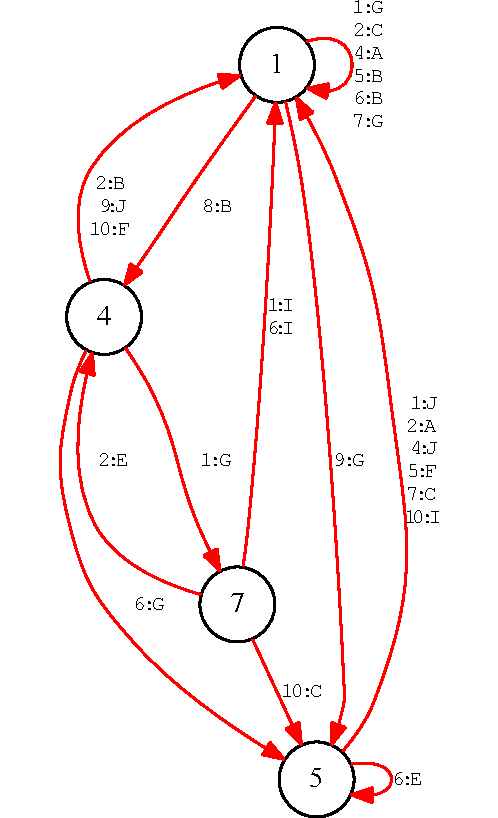
\includegraphics[height=2in]{random_alg-2}}
\end{figure}
\end{frame}

\section{Comparisons}
\begin{frame}
\frametitle{Poisson Random Tree}
\begin{tabular}{lr}
\begin{tabular}{c}
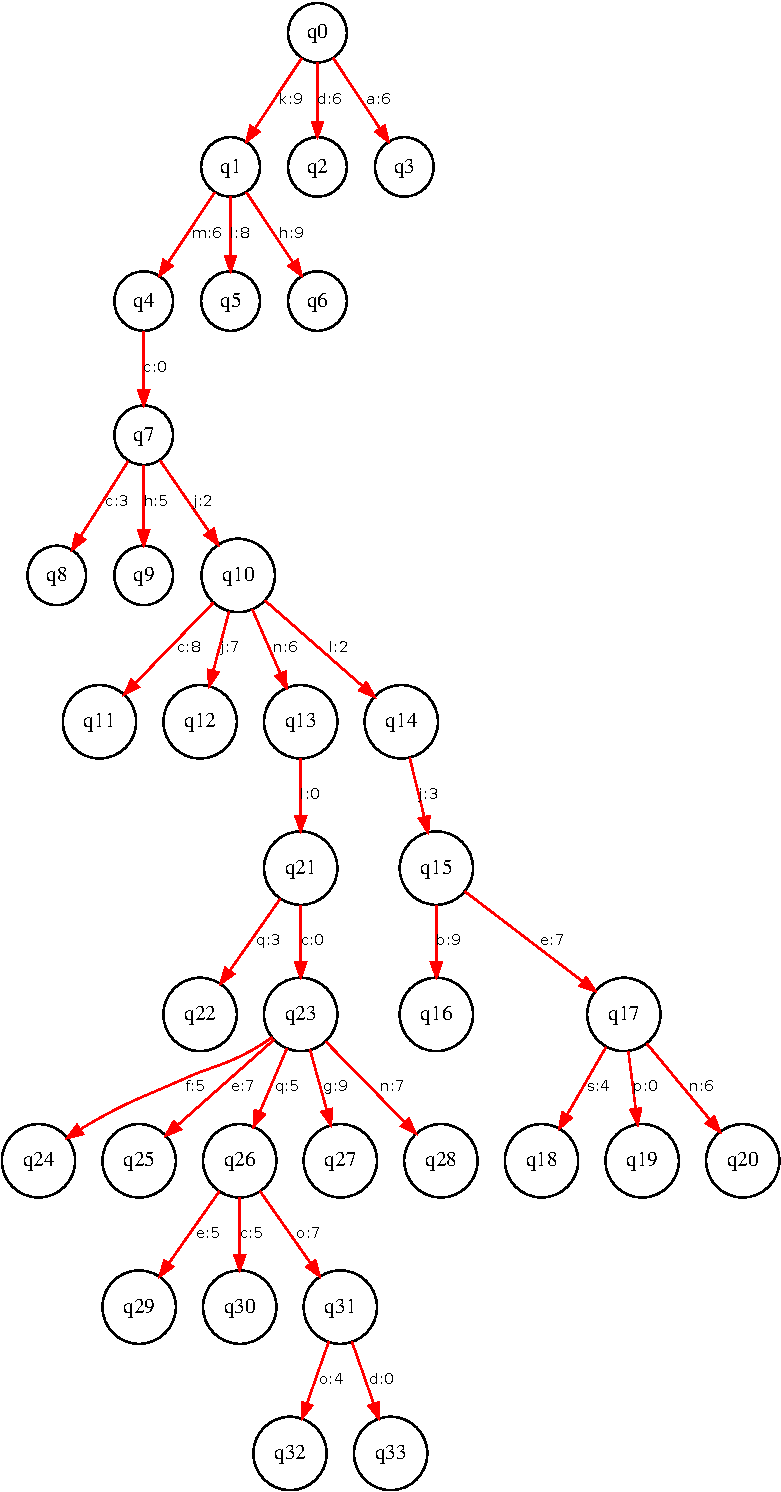
\includegraphics[width=1in]{big_tree.pdf}
\end{tabular}
&
\begin{tabular}{l}
  \parbox{2in}{
      Generated by recursively adding
      $X\sim\operatorname{Poisson(\lambda)}$   children to each new node.  
      Result is conditioned on process not terminating before depth $H$.\\
      
      Models a birth/death process where
      individuals continuously produce
      offspring at a rate of $\lambda$ per lifetime.      
      }
\end{tabular}
\end{tabular}
\end{frame}

\section{Comparisons}
\begin{frame}
\frametitle{Poisson Random Tree}
\begin{tabular}{lr}
\begin{tabular}{c}
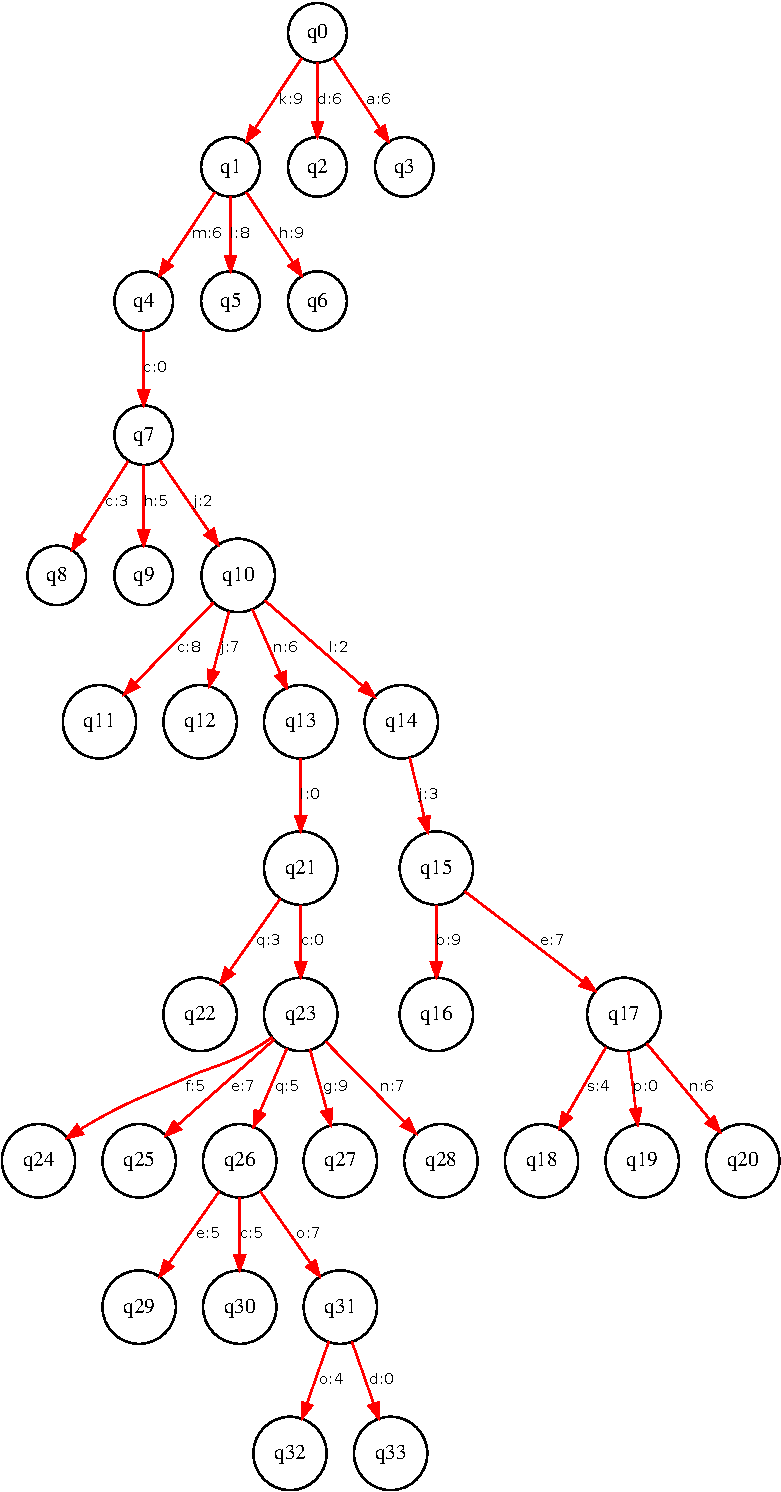
\includegraphics[width=1in]{big_tree.pdf}
\end{tabular}
&
\begin{tabular}{l}
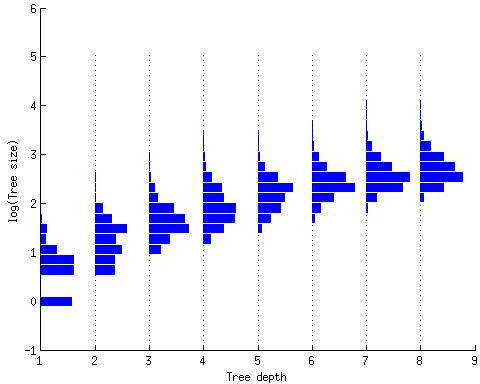
\includegraphics[height=2.5in]{poiss_size.jpg}
\end{tabular}
\end{tabular}
\end{frame}

\begin{frame}
\frametitle{Reduction Examples}
\begin{figure}
\centering
\subfigure[Original]{
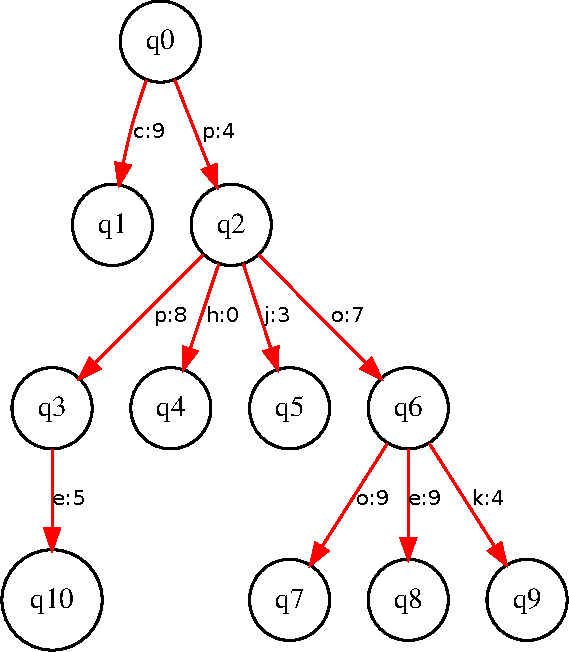
\includegraphics[scale=0.25]{orig.pdf}
}\\
\subfigure[Censi]{
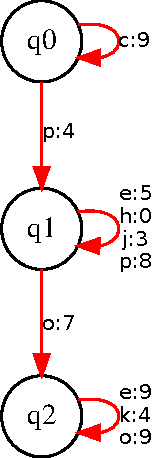
\includegraphics[scale=0.3, angle=20]{censi.pdf}\qquad
}
\subfigure[Josh]{
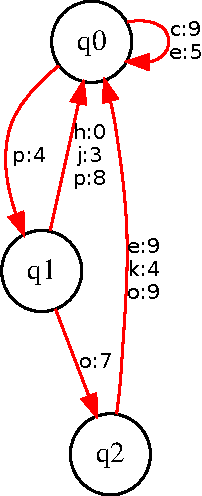
\includegraphics[scale=0.3, angle=20]{josh.pdf}\qquad
}
\subfigure[Alberto]{
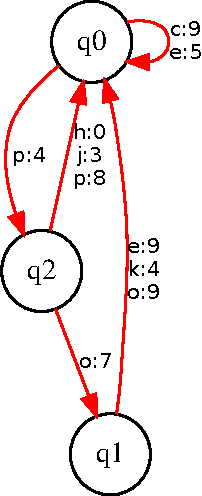
\includegraphics[scale=0.3, angle=20]{alberto.pdf}\qquad
}
\subfigure[Exact]{
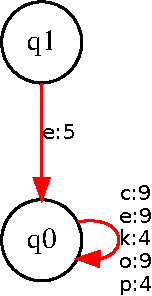
\includegraphics[scale=0.3, angle=20]{exact.pdf}
}
\end{figure}
\end{frame}

\begin{frame}
\begin{figure}
\centering
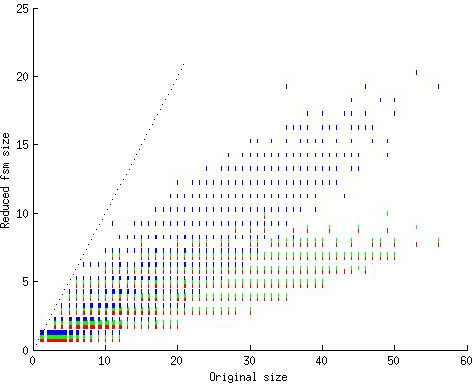
\includegraphics[height=3.4in]{poiss_orig.jpg}
\end{figure}
\end{frame}

\begin{frame}
\begin{figure}
\centering
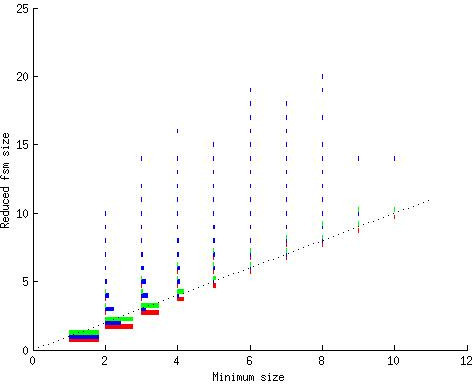
\includegraphics[height=3.4in]{poiss_exact.jpg}
\end{figure}
\end{frame}

\begin{frame}
\begin{figure}
\centering
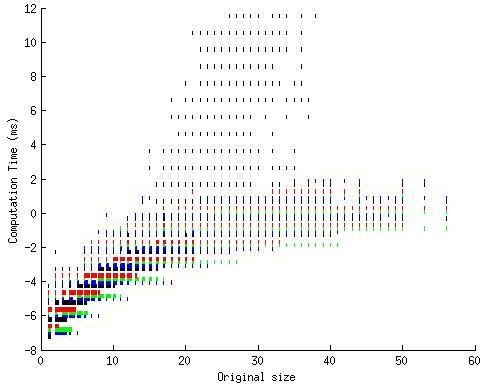
\includegraphics[height=3.4in]{poiss_time.jpg}
\end{figure}
\end{frame}

\begin{frame}
\frametitle{Pathological Tree}
\begin{figure}
\centering
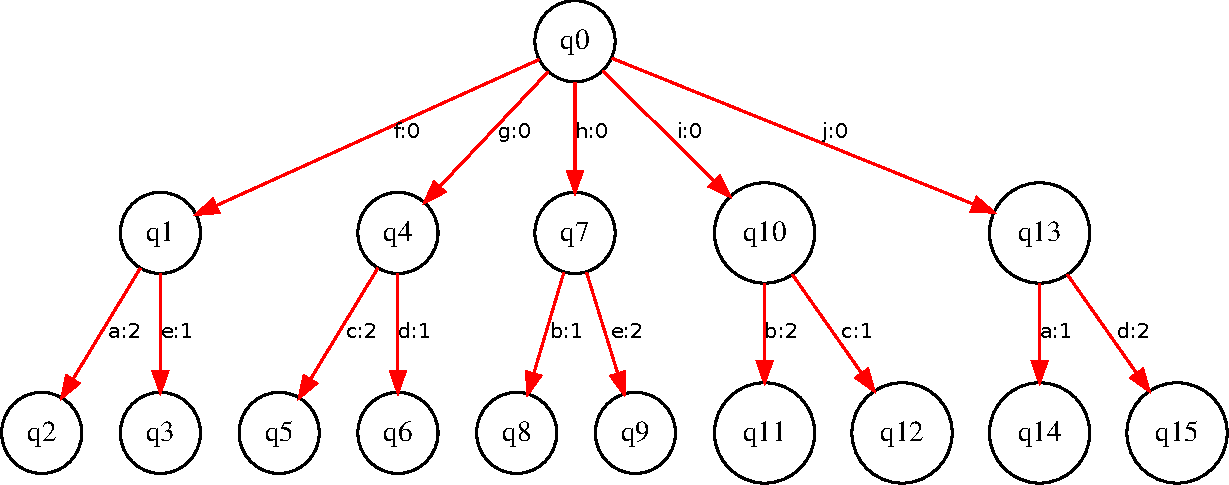
\includegraphics[width=4in]{big_patho_tree.pdf} 
\end{figure}
Each of the states at depth 1 is incompatible with exactly two others.  
This creates a distinction graph consisting of disjoint rings.
\end{frame}

\begin{frame}
\begin{figure}
\centering
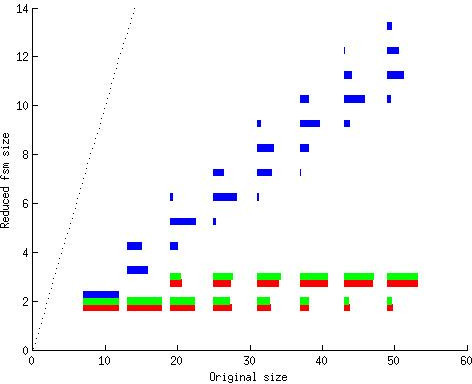
\includegraphics[height=3.4in]{patho_orig.jpg}
\end{figure}
\end{frame}

\begin{frame}
\begin{figure}
\centering
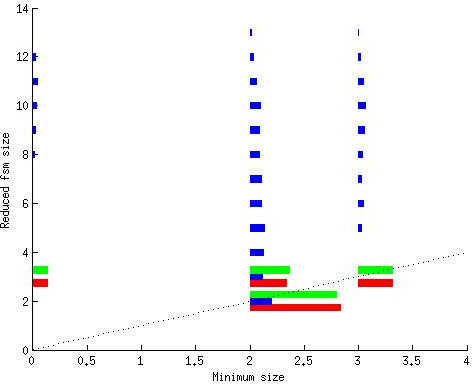
\includegraphics[height=3.4in]{patho_exact.jpg}
\end{figure}
\end{frame}

\begin{frame}
\begin{figure}
\centering
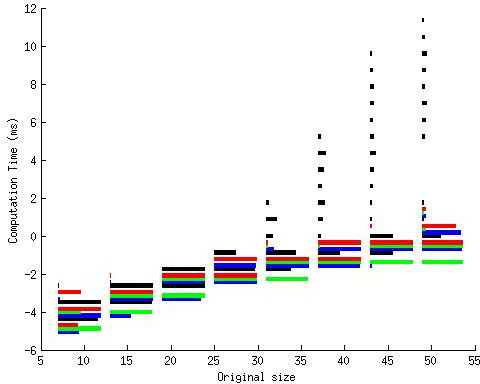
\includegraphics[height=3.4in]{patho_time.jpg}
\end{figure}
\end{frame}

%----------------------------------------------------------------------------------------

\end{document}